\documentclass{article}
\usepackage[utf8]{inputenc}
\usepackage{amsmath}
\usepackage{graphicx}
\usepackage[margin=1in]{geometry}
\usepackage{listings}
\usepackage{color}

\lstset{
  language=Matlab,
  basicstyle=\ttfamily\small,
  breaklines=true,
  keepspaces=true,
  numbers=left,
  numberstyle=\tiny,
  frame=tb,
  columns=fullflexible,
  showstringspaces=false,
  commentstyle=\color{green},
  keywordstyle=\color{blue}
} 

\title{ELCT 562: Laboratory Experiment \#2 [OFDM Transmission]}
\author{Jacob C. Vaught}
\date{April 7, 2024}

\begin{document}
\maketitle
\section*{Introduction to OFDM}
Orthogonal Frequency Division Multiplexing (OFDM) is a key modulation technique used in digital communication systems. It divides a high-data-rate modulating signal into several slower data rate substreams, each of which modulates a separate carrier frequency.

\subsection*{Mathematical Background}
The essence of OFDM lies in its use of orthogonal sub-carriers to carry data. Mathematically, the OFDM signal can be represented as a sum of these sub-carriers, each modulated by a data-bearing symbol. Given \(N\) sub-carriers, the OFDM signal \(s(t)\) over a symbol period \(T\) is:

\[
s(t) = \sum_{k=0}^{N-1} X_k e^{j2\pi f_k t}, \quad 0 \leq t < T
\]

where:
\begin{itemize}
    \item \(X_k\) represents the symbol carried by the \(k^{th}\) sub-carrier.
    \item \(f_k\) is the frequency of the \(k^{th}\) sub-carrier.
    \item \(N\) is the total number of sub-carriers.
    \item \(t\) represents time.
\end{itemize}

Orthogonality is achieved when the sub-carrier spacing (\(\Delta f\)) ensures that \(f_k = k\Delta f\) where \(\Delta f = \frac{1}{T}\), effectively preventing interference between the closely spaced sub-carriers in the frequency domain.

\subsection*{Practical Considerations}
In practice, OFDM's implementation hinges on the FFT and its inverse (IFFT), streamlining the modulation and demodulation processes. The IFFT is applied to convert the set of frequency-domain symbols \(\{X_0, X_1, ..., X_{N-1}\}\) into a time-domain signal, which is then transmitted over the channel. At the receiver, the FFT is used to demodulate the received time-domain signal back into the frequency domain for symbol detection.

\subsubsection*{Cyclic Prefix Addition}
A cyclic prefix (CP) is added to each OFDM symbol to guard against inter-symbol interference (ISI) caused by multipath propagation. The CP is a repetition of the end of the OFDM symbol appended to its beginning. If the CP length is \(L_{CP}\), the transmitted symbol, including the CP, can be expressed as \(x'_n = x_{(n \mod N)}\) for \(n = -L_{CP}, ..., N-1\).

\subsubsection*{Conversion from Bits to Multicarrier Signal and Back}
The conversion from a bitstream to an OFDM multicarrier signal entails:
\begin{enumerate}
    \item \textbf{Bit to Symbol Mapping:} Bits are mapped to symbols using a modulation scheme, e.g., QAM.
    \item \textbf{IFFT Processing:} Symbols are assigned to sub-carriers and converted to the time-domain via IFFT.
    \item \textbf{Cyclic Prefix Addition:} A CP is added to mitigate ISI and multipath effects.
\end{enumerate}

The receiver performs the inverse operations:
\begin{enumerate}
    \item \textbf{Cyclic Prefix Removal:} The CP is removed from the received signal.
    \item \textbf{FFT Processing:} The signal is converted back to the frequency domain using FFT.
    \item \textbf{Symbol Demapping:} Frequency-domain symbols are demapped back into bits.
\end{enumerate}

\subsubsection*{Channel Estimation and Equalization}
Channel conditions, including multipath effects and fading, are accounted for using pilot symbols for channel estimation. Equalization is performed on a per-subcarrier basis, facilitated by the FFT and IFFT operations, enabling efficient symbol detection and bit recovery in the presence of channel impairments.

\subsection*{Advantages of OFDM}
OFDM's structure provides significant advantages, including robustness to multipath fading and high spectral efficiency. Its ability to turn a frequency-selective fading channel into multiple flat-fading channels simplifies equalization and allows for flexible adaptation to channel conditions, making it a foundational technology in modern wireless communication systems.


\section*{Project Constraints and Mitigation Strategies}
This project focuses on designing an OFDM system under specific constraints, including a maximum signal bandwidth of 5 MHz and a minimum data rate of 7.5 Mbps, while supporting the transmission of 64 text characters in a packet.

\subsection*{Understanding Constraints}
\begin{itemize}
    \item \textbf{Bandwidth Limitation:} The system's total bandwidth must not exceed 5 MHz.
    \item \textbf{Data Rate Requirement:} The system must achieve a data rate of at least 7.5 Mbps.
    \item \textbf{Packet Support:} The system must accommodate packets that support 64 text characters.
\end{itemize}

\subsection*{Mitigation Strategies}
Several strategies can be employed to meet these constraints, including optimizing the modulation scheme, carefully selecting the number of subcarriers, and managing the cyclic prefix length.

\section*{Our Solution and Results}
After extensive analysis, we chose a 16-QAM modulation scheme with 128 channels and a subcarrier spacing of 25 kHz. This setup offered a compromise between bandwidth efficiency and robustness against channel imperfections.

\subsection*{Solution Description}
Our OFDM system utilizes a cyclic prefix length of one-fourth the symbol duration to combat inter-symbol interference. This choice ensures that our system not only meets but exceeds the minimum data rate requirement, achieving a data rate of 10.24 Mbps within the 5 MHz bandwidth constraint.

\subsection*{Results and Discussion}
The chosen parameters led to a system that not only satisfies the project's constraints but also offers a buffer in terms of bandwidth and data rate, allowing for future scalability and robustness in varying channel conditions.

\begin{equation}
    \text{Data Rate} = \frac{N \times \text{Bits per Symbol}}{T_{\text{Symbol}} + T_{\text{CP}}}
\end{equation}

\section*{OFDM System Performance and Characteristics}

This section presents the analysis of the OFDM system under study, showcasing the estimated Carrier Frequency Offset (CFO), the channel frequency response, the received constellation after equalization, and several key parameters of the OFDM transmission.

\subsection*{Estimated CFO}
The estimated Carrier Frequency Offset (CFO) in the system is found to be \(-22.936522\) Hz.

\subsection*{Channel Frequency Response}
The estimated channel frequency response is depicted in the figure below. This response gives insight into how different frequency components of the signal are affected by the channel.
\begin{figure}[h!]
  \centering
  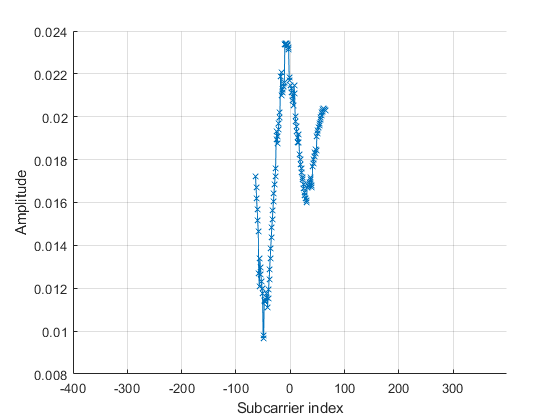
\includegraphics[width=0.6\textwidth]{channel_response.png}
  \caption{Estimated Channel Frequency Response}
\end{figure}

\subsection*{Received Constellation after Equalization}
The constellation diagram after equalization is shown below, illustrating the effectiveness of the equalization process in correcting for channel impairments.
\begin{figure}[h!]
  \centering
  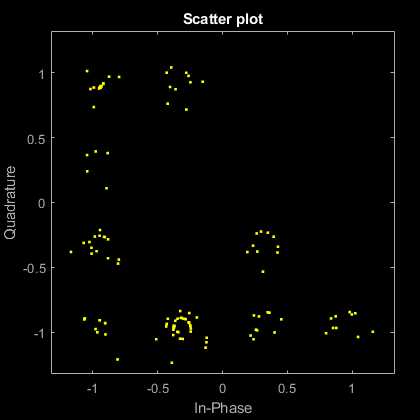
\includegraphics[width=0.5\textwidth]{constellation.png}
  \caption{Received Constellation after Equalization}
\end{figure}

\subsection*{System Parameters}
The following parameters were observed or calculated for the OFDM system under analysis:

\begin{itemize}
    \item \textbf{Signal Bandwidth:} \(3,200,000\) Hz
    \item \textbf{Sample Rate:} \(20,000,000\) Hz
    \item \textbf{Packet Size:} \(2000\) samples
    \item \textbf{Subcarrier Spacing:} \(25,000\) Hz
    \item \textbf{Cyclic Prefix Duration:} \(0.000010\) seconds
\end{itemize}

\subsection*{Received Text}
The text received after demodulation and decoding is shown to be:

\begin{verbatim}
Hello WorldHello WorldHello WorldHello WorldHello World
\end{verbatim}

\section*{Receiver Algorithms for Synchronization}

Synchronization is a crucial step in OFDM receivers, ensuring the correct timing and frequency alignment of the received signal for successful demodulation and decoding. This section delves into the synchronization algorithms employed in our OFDM system, focusing on the techniques used for achieving time and frequency synchronization, specifically Carrier Frequency Offset (CFO) estimation.

\subsection*{Time Synchronization}

Time synchronization involves identifying the start of an OFDM symbol within the received signal. It is essential for removing the cyclic prefix correctly and aligning the FFT window. The algorithm utilizes the cyclic prefix's properties by correlating the signal with a delayed version of itself, exploiting the inherent redundancy:

\[
P(n) = \sum_{m=0}^{L-1} y(n+m) \cdot y^*(n+m+L)
\]

\[
R(n) = \sum_{m=0}^{L-1} |y(n+m+L)|^2
\]

\[
\text{Metric}(n) = \frac{|P(n)|^2}{R(n)^2}
\]

A peak in this metric indicates the start of an OFDM symbol. The choice of \(L\), which is typically set to the cyclic prefix length, plays a crucial role in the robustness of the synchronization process.

% Placeholder for figure or algorithmic flowchart
\begin{figure}[h!]
  \centering
  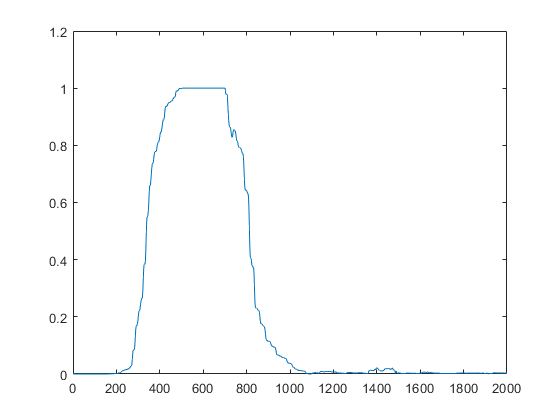
\includegraphics[width=0.8\textwidth]{sync.png}
  \caption{Synchronization view}
\end{figure} 

\subsection*{Carrier Frequency Offset (CFO) Estimation}

The CFO arises from a mismatch in the carrier frequencies of the transmitter and receiver oscillators, leading to a rotation of the constellation points in the complex plane. Accurate CFO estimation and correction are vital for coherent demodulation. The estimated CFO, based on the phase difference between the received signal and its delayed version, is given by:

\[
\hat{f}_{\text{CFO}} = -\frac{\angle P(n_{\text{chosen}})}{2\pi L} \cdot f_{\text{sample}}
\]

where \(n_{\text{chosen}}\) is the sample index identified during time synchronization as the beginning of an OFDM symbol.

\subsection*{Implementation and Results}

In our implementation, synchronization signals and a predetermined sequence known at the receiver were used to facilitate these algorithms. The effectiveness of the synchronization and CFO correction processes are critical for the overall system performance, as depicted in the following results:

\begin{itemize}
    \item Estimated CFO: -22.936522 Hz
    \item Signal Bandwidth: 3,200,000 Hz
    \item Sample Rate: 20,000,000 Hz
    \item Packet Size: 2000 samples
    \item Subcarrier Spacing: 25,000 Hz
    \item Cyclic Prefix Duration: 0.000010 seconds
    \item Received Text: ``Hello WorldHello WorldHello WorldHello WorldHello World''
\end{itemize}

The presented synchronization strategy effectively aligns the receiver, ensuring the integrity of the received OFDM symbols for further processing and decoding.


\section*{Development and Simulation of the OFDM System}

In the initial phase of our project, we developed a lab-based transmitter/receiver pair utilizing 16-QAM modulation with 52 subcarriers. To extend our research and facilitate future works, we subsequently developed a simulation model of our system. This model aimed to accurately reflect the system's performance and provide a basis for further enhancements.

As part of our system's evolution, we increased the number of subcarriers to 128 to improve the system's capacity and robustness. This adjustment necessitated the development of a new synchronization sequence. To meet this requirement, we utilized a Golay sequence generator, known for its optimal correlation properties, making it highly suitable for our synchronization needs.

Below, we attach the MATLAB code for the key components of our project. This includes the simulation model of our OFDM system, the Golay sequence generator used for synchronization, and the practical implementations of both the transmitter and receiver as realized in our lab setup.

\subsection*{Simulation Model for the OFDM System}
The simulation model encapsulates our initial system design with 52 subcarriers and extends it to accommodate 128 subcarriers, laying the groundwork for future enhancements and studies.

\lstinputlisting{Transmitter_simulation_code.m} % MATLAB code for the transmitter simulation

\subsection*{Golay Sequence Generator}
To adapt to the increased number of subcarriers, a Golay sequence generator was developed. This sequence plays a crucial role in the synchronization process of our OFDM system.

\lstinputlisting{generateGolaySequence.m} % MATLAB code for generating Golay sequence

\subsection*{Lab-Based Transmitter Implementation}
This section includes the MATLAB code for our lab-implemented transmitter, which has been crucial in our practical experiments and testing phases.

\lstinputlisting{transmitter.m} % MATLAB code for the lab transmitter

\subsection*{Lab-Based Receiver Implementation}
Similarly, this section provides the MATLAB code for our lab-implemented receiver. Together with the transmitter, this forms the backbone of our practical OFDM system experimentation.

\lstinputlisting{receiver_lab2.m} % MATLAB code for the lab receiver


\end{document}
